
DOM objects are hierarchically organized into a DOM tree with the topnode of a XML document as the root object of the DOM tree. Every part of a XML document correspondes to a DOM object: The following code snippet of a XML document is mapped to the tree shown in figure \ref{fig:simpleDomTree}.

\begin{verbatim}
<html>
 <head>
  <title>DocumentTitle</title>
 </head>
 <body>
  <h1 id="aHeading">Heading</h1>
  <br />
  <p id="aParagraph" style="fontFamily:sans-serif;">Content</p>
 </body>
</html>
\end{verbatim}

\begin{figure}[htbp]
	\centering
		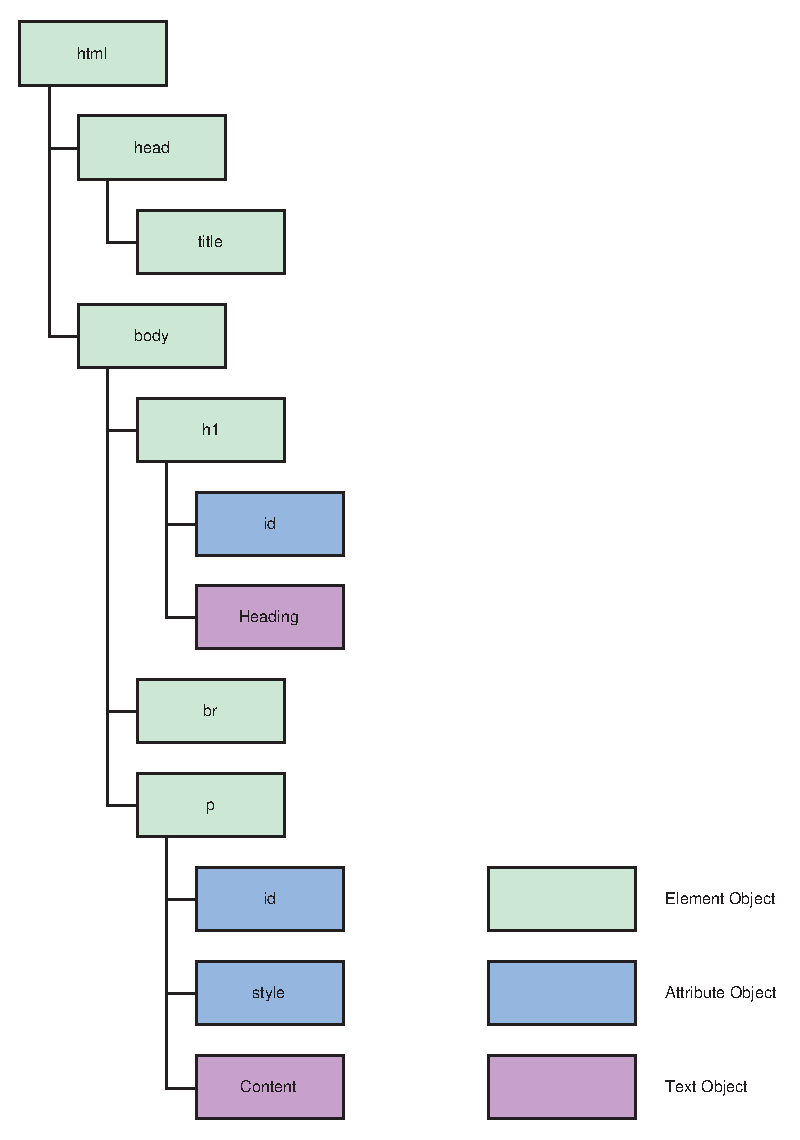
\includegraphics[scale=0.5]{simpleDomTree}
	\caption{SDT}
	\label{fig:simpleDomTree}
\end{figure}

The figure showes three types of DOM 'classes': 

\begin{enumerate}
	\item Element objects, these correspond to XML tags and are characterized by there type, e.g. a \texttt{h1} or a \texttt{title}.
	\item Attribute objects, these correspond to XML attributes and are name-value pairs, e.g. the paragraphs \texttt{style} value is \texttt{Heading}.
	\item Text objects, the part of the document between the tags that is the (unstructured) content of document.
	
\end{enumerate}

Properties and methods available for these DOM classes are also definined in the DOM standard; DOM for example defines that each element node may have an attribute \texttt{id} and that every element node supports the method \texttt{appendChild} that expects another node as argument and attaches this node to the node the method is invoked on.

